\chapter{Ansatz und Entwurf}
\label{Ansatz}

% ---------------------------------------------------------------------------
% Leitfaden des Betreuers (nicht Teil des Fließtextes, dient als Schreibhilfe):
% In diesem Kapitel wird gezeigt, WIE die im letzten Kapitel ermittelten
% generellen Ziele realisiert werden. Bei konzeptionellen Arbeiten erfolgt das
% durch einen Software- oder Softwarearchitekturentwurf. Dieses Kapitel ist der
% wichtigste Teil der Arbeit -- hier muss klar argumentiert und es müssen
% Alternativen bewertet werden. Entwurfsentscheidungen müssen begründet werden,
% sodass sie nachvollziehbar sind. Immer muss klar werden,
% inwiefern der Gesamtentwurf und seine Einzelaspekte die Forschungsfrage lösen.
% Anmerkungen 22.09.: erst den Ansatz präsentieren, dann Ziele/Anforderungen;
% Teilaspekte statt Entscheidungskapitel; Entscheidungen "on the go".
% ---------------------------------------------------------------------------

% GEÄNDERT: Kapiteleinleitung an die neue Reihenfolge angepasst (Lösung zuerst, Betreueranmerkung S1)
Aufbauend auf der in Kapitel~\ref{StandDerForschung} hergeleiteten Forschungslücke wird in diesem Kapitel der Ansatz des Analyseframeworks beschrieben. Beschrieben wird dabei der Zielentwurf, dessen prototypische Umsetzung Gegenstand von Kapitel~\ref{Implementierung} ist. Die Darstellung beginnt mit der Lösung im Gesamtkontext, leitet daraus die Ziele sowie Anforderungen ab und gibt anschließend einen Überblick über die Architektur. Im Anschluss werden die vier Teilaspekte des Ansatzes einzeln erläutert, wobei jede Entwurfsentscheidung an der Stelle begründet wird, an der sie erforderlich ist, und gegen die jeweils betrachteten Alternativen abgewogen wird.

\section{Lösung im Gesamtkontext}
\label{sec:loesung}

% GEÄNDERT: Platzhalter durch Abbildung ersetzt (draw.io, Quelldatei Grafiken/drawio/abb3_1_loesung.drawio); zeigt den Zielentwurf (R7); direkt unter der Überschrift, damit die Abbildung auf der ersten Seite des Kapitels steht (Meeting-Notiz M6)
\begin{figure}[H]
	\centering
	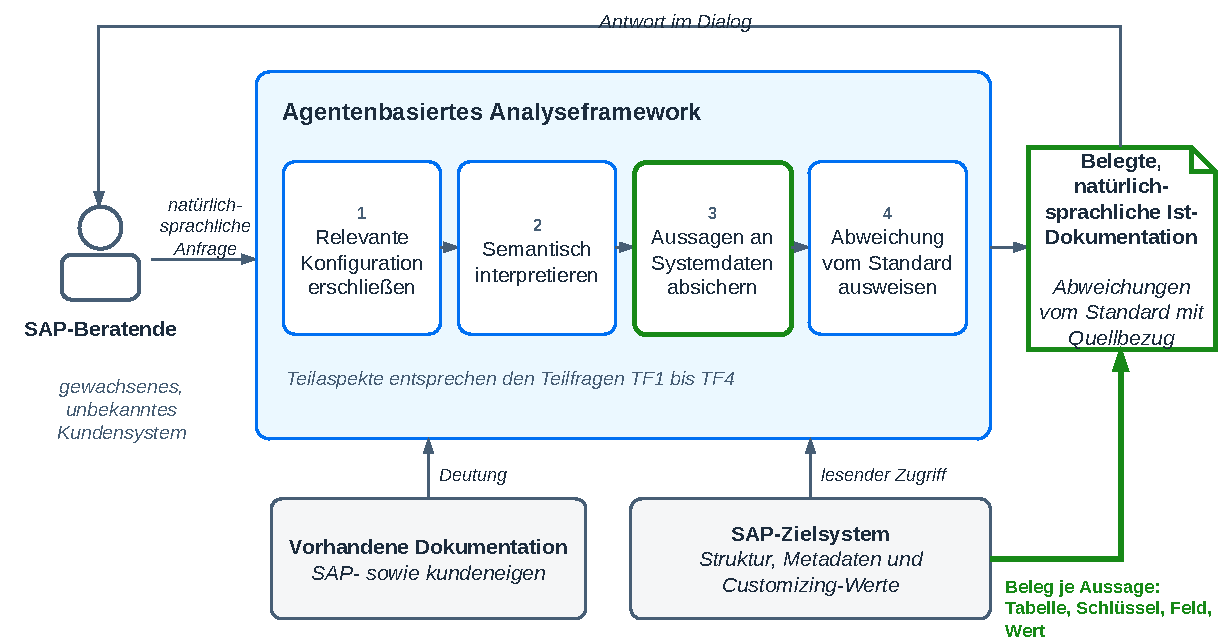
\includegraphics[width=\linewidth]{Grafiken/abb3_1_loesung.pdf}
	\caption{Konzeptioneller Aufbau des agentenbasierten Analyseframeworks sowie der Datenfluss einer Analyseanfrage von der Fragestellung bis zur belegten Antwort (eigene Darstellung).}
	\label{fig:ansatz-ueberblick}
\end{figure}

% GEÄNDERT: RAG durch Grounding ersetzt (einheitliche Terminologie mit 2.2.1); Zugriff auf Werte ergänzt, da der Ansatz neben Struktur und Metadaten auch die Customizing-Werte liest
Der Ansatz besteht in einem agentenbasierten Analyseframework, das den
funktionalen Ist-Zustand eines SAP-Systems ausgehend von einer
natürlichsprachlichen Analyseanfrage erschließt und die identifizierten
Abweichungen vom Herstellerstandard in einer fachlich belastbaren,
natürlichsprachlichen Dokumentation zusammenführt. Abbildung~\ref{fig:ansatz-ueberblick}
zeigt den konzeptionellen Aufbau sowie den Datenfluss einer Anfrage von der
Fragestellung bis zur belegten Antwort. Ausgehend von der Analyseanfrage greift
ein agentenbasierter Orchestrator über eine standardisierte Schnittstelle des
Model Context Protocol (MCP) lesend auf die Struktur- und Metadatenebene sowie
die Customizing-Werte des Zielsystems zu, erschließt die zusammenhängenden Customizing-Tabellen und deren
Abweichungen vom Standard und überführt diese mittels eines Sprachmodells in
eine semantische Interpretation, die durch Grounding
an den abgerufenen Systemdaten abgesichert wird. Das Ergebnis besteht in einem
Dokument, das den Ist-Zustand mit den erkannten Abweichungen beschreibt.


Der Verarbeitungsweg gliedert sich in drei aufeinander aufbauende Ebenen, die
jeweils eine eigene Teilaufgabe erfüllen und daher je eigene Fehlerarten
aufweisen. Zunächst erfolgt auf der Ebene des Retrievals das Schema-Linking, das
aus einem sehr großen Datenkatalog die für eine Anfrage relevanten Tabellen
bestimmt, da das vollständige Schema aus Gründen des Kontextfensters nicht als
Eingabe dienen kann. Im Anschluss erfolgt auf der Ebene des Zugriffs die lesende
Abfrage der ausgewählten Struktur- und Metadaten über die MCP-Schnittstelle.
Abschließend erfolgt auf der Ebene des Groundings die Absicherung der erzeugten
Aussagen, indem jede Aussage nachweisbar an die abgerufenen Quelldaten gebunden
und bei nicht tragender Evidenz eine begründete Enthaltung ausgelöst wird. Diese
begriffliche Trennung von Retrieval, Zugriff und Grounding bildet die
Ordnungsstruktur, entlang derer die Entwurfsentscheidungen in
Abschnitt~\ref{sec:teilaspekte} behandelt werden. % GEÄNDERT: Verweis auf neuen Abschnitt

% NEU: Teilaspekte vorab benannt und aus dem Stand der Forschung abgeleitet (Meeting-Notizen M7 sowie R7: "der Ansatz soll sich aus dem Related Work ergeben")
Innerhalb dieser Ebenen besteht der Ansatz aus vier Teilaspekten, die jeweils einer Teilfrage der Forschungsfrage entsprechen. Der erste Teilaspekt erschließt die zu einer Anfrage relevante Konfiguration, der zweite interpretiert deren Werte semantisch, der dritte sichert jede Aussage an den Systemdaten ab, und der vierte weist die Abweichungen vom Herstellerstandard aus. Keiner dieser Teilaspekte wird neu erfunden. Jeder übernimmt vielmehr ein in Abschnitt~\ref{sec:stand-forschung} betrachtetes Verfahren und erweitert es um das, was die Customizing-Ebene zusätzlich erfordert. Tabelle~\ref{tab:teilaspekte} stellt diese Herleitung gegenüber.

\begin{table}[htbp]
\centering
\caption{Herleitung der Teilaspekte aus dem Stand der Forschung}
\label{tab:teilaspekte}
\small
\begin{tabular}{p{2.2cm}p{0.8cm}p{4.2cm}p{4.6cm}}
\toprule
\textbf{Teilaspekt} & \textbf{TF} & \textbf{Übernommen aus} & \textbf{Erweiterung für die Customizing-Ebene} \\
\midrule
Erschließen & TF1 & iterative, agentengesteuerte Exploration des Schemas \cite{wang_autolink_2026}; Ableitung der Tabellenbeziehungen aus dem DDIC \cite{berti_generic_2023} & Vorfilterung des Suchraums über die Auslieferungsklasse; semantische Suche als Werkzeug hinter der Schnittstelle \\
Interpretieren & TF2 & Anreicherung um Bezeichnersemantik \cite{cai_columbo_2025, wretblad_synthetic_2024}; sprachmodellgestützte Dokumentation \cite{diggs_leveraging_2024} & deterministische Auflösung von Schlüsselwerten über Prüf- und Texttabellen sowie von Merkmalen \\
Absichern & TF3 & mitgelieferte Belegabfrage \cite{theologitis_thucy_2026}; Prüfung vor der Ausgabe \cite{allemang_increasing_2025}; Enthaltung \cite{somov_confidence_2025} & Belegeinheit aus Tabelle, Schlüssel, Feld und Wert; Prüfung im Programmcode statt im Prompt \\
Abweichung ausweisen & TF4 & Standardnähe \cite{sekatzek_messung_2009}; tabellarischer Customizing-Abgleich \cite{sap_customizing_abgleich} & fachliche Deutung der ermittelten Abweichung \\
\bottomrule
\end{tabular}
\end{table}

% GEÄNDERT: Begründung des Fokus mit "weil" an die Lücke gebunden (Meeting-Notiz M8); Verweis korrigiert (vorher undefiniertes Label "Forschungsstand")
Der Betrachtungsschwerpunkt liegt auf der Customizing-Ebene. Dies liegt darin
begründet, dass die fachliche Bedeutung einer Customizing-Einstellung nicht aus
einem einzelnen Artefakt hervorgeht, sondern aus dem Zusammenspiel der
konfigurierten Werte mit der interpretierenden Standardlogik resultiert, und dass
gerade diese semantische Interpretation der Customizing-Ebene nach dem in
Abschnitt~\ref{sec:forschungsluecke} dargelegten Kenntnisstand unbesetzt verbleibt.
Kundeneigener ABAP-Code wird kontextgebunden herangezogen, um
Customizing-Abweichungen zu erklären, nicht jedoch als eigenständiges
Analyseobjekt behandelt.

% NEU: durchgängiges Beispiel im Gesamtkontext (Meeting-Notiz M11)
Am durchgängigen Beispiel lässt sich der Ablauf wie folgt nachvollziehen. Die Anfrage, welche Abwesenheitsarten Auszubildende beantragen dürfen, führt im ersten Teilaspekt auf die Customizing-Tabelle, welche die beantragbaren Arten je Regelgruppe festlegt, sowie auf das Merkmal, das die Regelgruppe bestimmt. Im zweiten Teilaspekt wird die Gruppe der Auszubildenden über dieses Merkmal einer Regelgruppe zugeordnet, und die zugehörigen Schlüsselwerte werden über die Texttabelle in Bezeichnungen überführt. Der dritte Teilaspekt gewährleistet, dass jede genannte Abwesenheitsart mit der Tabellenzeile belegt ist, aus der sie stammt, und dass eine nicht eindeutig bestimmbare Regelgruppe zu einer Rückfrage statt zu einer Vermutung führt. Der vierte Teilaspekt weist schließlich aus, welche dieser Einträge vom Auslieferungszustand abweichen.

\section{Ziele und Anforderungen}
\label{sec:ziele-anforderungen}

% VERSCHOBEN aus 3.1 und GEÄNDERT: Teilziele an die vier Teilfragen angeglichen (Ziele als Teil des Ansatzes, Betreueranmerkung S1)
Ziel des Ansatzes ist es, die Customizing-Ebene zu erschließen, semantisch zu interpretieren, jede Aussage an den Systemdaten zu belegen sowie Abweichungen vom SAP-Standard auszuweisen und das Ergebnis in eine natürlichsprachliche Dokumentation zu überführen. Diese Teilziele entsprechen unmittelbar den in Abschnitt~\ref{sec:problem-ff} formulierten Teilfragen und strukturieren den gesamten Entwurf: Die Erschließung gewährleistet, dass die für eine Anfrage relevanten Konfigurationen überhaupt gefunden werden; die semantische Interpretation stellt sicher, dass deren fachliche Bedeutung erschlossen und nicht allein der technische Wert wiedergegeben wird; die Belegung gewährleistet, dass jede Aussage nachprüfbar bleibt; der Ausweis der Abweichung macht das Ergebnis schließlich für die fachliche Einordnung im Rahmen von Transformationsprojekten nutzbar. Die Absicherung dieser Aussagen gegen nicht gedeckte Interpretationen bildet dabei die entscheidende Abgrenzung des Ansatzes von einer generischen Retrieval-Augmented Generation.

\subsection{Funktionale Anforderungen}
\label{subsec:anf-funktional}

% GEÄNDERT/NEU (R12): Skizze zu nummerierten Anforderungen mit Bezug zur Teilfrage ausformuliert
Die funktionalen Anforderungen beschreiben, welche Leistungen das Framework erbringen muss, um die Teilfragen zu beantworten. Sie umfassen folgende Punkte:
\begin{enumerate}
	\item[\textbf{FA1}] \textbf{Natürlichsprachliche Anfrage:} Das Framework nimmt Anfragen in natürlicher Sprache entgegen und ermöglicht Folgefragen im Dialog. (alle TF)
	\item[\textbf{FA2}] \textbf{Erschließung ohne vollständiges Schema:} Das Framework bestimmt die für eine Anfrage relevanten Customizing-Tabellen sowie Felder, ohne das vollständige Schema als Eingabe zu benötigen. (TF1)
	\item[\textbf{FA3}] \textbf{Lesender Zugriff:} Das Framework liest Struktur, Metadaten sowie Werte der ermittelten Tabellen und bei Bedarf den Quelltext zugehöriger Eigenentwicklungen. (TF1, TF2)
	\item[\textbf{FA4}] \textbf{Klartextauflösung:} Das Framework überführt Schlüsselwerte über die im DDIC gepflegten Beziehungen in ihre Bezeichnungen und löst Merkmale auf. (TF2)
	\item[\textbf{FA5}] \textbf{Belegpflicht:} Jede Aussage trägt den Verweis auf die Tabellenzeile sowie die Abfrage, aus der sie stammt, und interpretierende Aussagen sind als solche gekennzeichnet. (TF3)
	\item[\textbf{FA6}] \textbf{Enthaltung:} Reicht die Evidenz für eine Aussage nicht aus, so wird die Aussage nicht erzeugt und die offene Frage an den Nutzer zurückgegeben. (TF3)
	\item[\textbf{FA7}] \textbf{Ausweis der Abweichung:} Das Framework kennzeichnet, welche Einträge vom Auslieferungszustand abweichen, und deutet diese Abweichungen fachlich. (TF4)
	\item[\textbf{FA8}] \textbf{Ergebnisdokument:} Die belegten Aussagen mehrerer Anfragen lassen sich zu einer strukturierten Ist-Dokumentation zusammenführen. (alle TF)
\end{enumerate}

\subsection{Nicht-funktionale Anforderungen und Randbedingungen}
\label{subsec:anf-nichtfunktional}

% GEÄNDERT: Gedankenstrich-Einschub aufgelöst; Anforderungen nummeriert und begründet (R12)
Die nicht-funktionalen Anforderungen legen die Qualitätsmerkmale des Entwurfs fest:
\begin{enumerate}
	\item[\textbf{NFA1}] \textbf{Nachvollziehbarkeit:} Der Weg von der Anfrage zur Aussage ist über die aufgerufenen Werkzeuge sowie die abgesetzten Abfragen rekonstruierbar, da ein fachkundiger Nutzer eine Aussage andernfalls nicht prüfen kann.
	\item[\textbf{NFA2}] \textbf{Austauschbarkeit des Sprachmodells:} Das verwendete Modell lässt sich ohne Änderung der übrigen Architektur ersetzen, da die Entwicklung der Modelle schneller verläuft als die Bearbeitungszeit der Arbeit.
	\item[\textbf{NFA3}] \textbf{Skalierbarkeit:} Die Erschließung bleibt auch bei einem Bestand von mehreren Tausend Customizing-Tabellen funktionsfähig, da das Data Dictionary eines SAP-Systems zehntausende Tabellen umfasst.
	\item[\textbf{NFA4}] \textbf{Reproduzierbarkeit:} Entscheidungen, die sich deterministisch aus den Metadaten ableiten lassen, werden nicht dem Sprachmodell überlassen, sodass sie für jeden Lauf identisch ausfallen.
\end{enumerate}

Neben diesen Anforderungen unterliegt der Entwurf drei Randbedingungen, die nicht aus der Zielsetzung der Arbeit, sondern aus der Umgebung des Kooperationspartners sowie aus dem Untersuchungsgegenstand resultieren. Die erste Randbedingung betrifft die Betriebsplattform: Die Lösung ist innerhalb der von der mmmake GmbH bereitgestellten SAP Business Technology Platform (BTP) zu realisieren, deren Konnektivitätsstrukturen den technischen Rahmen des Zugriffs auf das Zielsystem festlegen und nicht Gegenstand einer eigenen Entwurfsentscheidung sind. Die zweite Randbedingung betrifft die Zugriffsart: Sämtliche Zugriffe auf das Quellsystem erfolgen ausschließlich lesend. Dies liegt darin begründet, dass der Untersuchungsgegenstand der Ist-Zustand eines gewachsenen Systems ist und ein schreibender Zugriff den zu beschreibenden Zustand verändern würde. Die dritte Randbedingung betrifft die Datenbasis: Als Untersuchungsgegenstand steht ein einzelnes SAP-System zur Verfügung, sodass sämtliche empirischen Aussagen zunächst an dessen Ausprägung gebunden sind. Entwurfsentscheidungen, die sich auf eine dieser Randbedingungen stützen, sind als bedingt zu verstehen, da sie bei veränderter Umgebung anders ausfallen könnten.
% Die technische Ausführung der BTP-Randbedingung (.dest-Proxy) wird in Kapitel 4 beschrieben.

\section{Architekturüberblick}
\label{sec:architektur-ueberblick}

% GEÄNDERT: Einleitung angepasst und Architekturdiagramm ergänzt (draw.io, Grafiken/drawio/abb3_2_architektur.drawio)
Auf Grundlage der zuvor definierten Anforderungen gibt dieser Abschnitt einen Überblick über die Gesamtarchitektur des Analyseframeworks, die in Abbildung~\ref{fig:architektur} dargestellt ist. Das System gliedert sich in eine Nutzerschnittstelle, einen agentenbasierten Orchestrator, einen über das Model Context Protocol angebundenen Werkzeugserver, die lesende Anbindung des Zielsystems sowie die Bereitstellung des Sprachmodells und der Einbettungsverfahren über den SAP Generative AI Hub.

\begin{figure}[htbp]
	\centering
	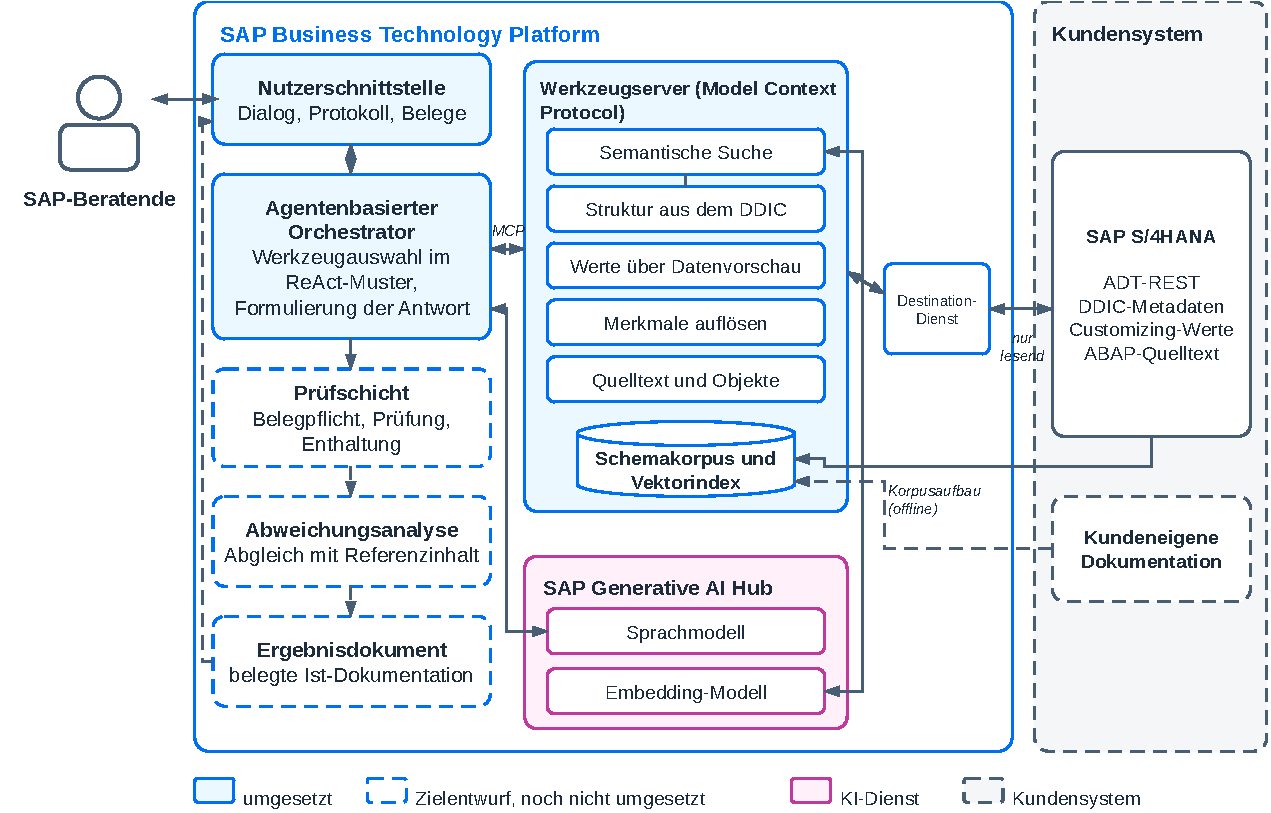
\includegraphics[width=\linewidth]{Grafiken/abb3_2_architektur.pdf}
	\caption{Architektur des Analyseframeworks; gestrichelt dargestellte Komponenten sind Teil des Zielentwurfs und im Prototyp noch nicht umgesetzt (eigene Darstellung im Stil der SAP-Referenzarchitekturen \cite{sap_architecture_center}).}
	\label{fig:architektur}
\end{figure}

% NEU (R12): Beschreibung der Komponenten und ihrer Zuordnung zu den Ebenen
Der Orchestrator nimmt die Anfrage entgegen, wählt die aufzurufenden Werkzeuge aus und formuliert aus deren Ergebnissen die Antwort. Der Werkzeugserver kapselt sämtliches Wissen darüber, wie die Metadaten sowie Werte eines SAP-Systems aufzufinden und zu lesen sind, und stellt dieses dem Orchestrator als klar abgegrenzte Werkzeuge bereit. Er enthält hierzu den aus dem Data Dictionary aufgebauten Schemakorpus samt Vektorindex, über den die semantische Suche erfolgt. Der Zugriff auf das Zielsystem erfolgt über die REST-Schnittstelle der ABAP Development Tools, wobei die Verbindung über die Konnektivitätsdienste der BTP hergestellt wird. Zwischen dem Orchestrator und der Ausgabe liegen die Prüfschicht sowie die Abweichungsanalyse, die in den Abschnitten~\ref{subsec:ta-absichern} und \ref{subsec:ta-abweichung} beschrieben werden.

% NEU (Textbaustein 14.09.2026): Rolle des Sprachmodells im Ablauf
Diese Aufteilung legt fest, an welchen Stellen das Sprachmodell wirkt. Es wirkt ausschließlich bei der Auswahl der Werkzeuge sowie bei der Formulierung der Antwort. An keiner Stelle bestimmt es, welche Daten als vorhanden gelten, da sowohl die semantische Suche als auch der lesende Zugriff sowie die Prüfung deterministisch außerhalb des Modells erfolgen. Dies ist die architektonische Voraussetzung dafür, dass eine Aussage an die Systemdaten gebunden werden kann.

\section{Teilaspekte des Ansatzes}
\label{sec:teilaspekte}

% GEÄNDERT: Einleitung umgestellt von "Entwurfsentscheidungen" auf "Teilaspekte", Entscheidungen werden innerhalb der Teilaspekte begründet (Betreueranmerkung S2)
Die folgenden Abschnitte beschreiben die vier Teilaspekte des Ansatzes. Jeder Abschnitt benennt zunächst die Teilfrage, die er adressiert, sowie das Verfahren, das er aus dem Stand der Forschung übernimmt, und beschreibt anschließend die eingesetzte Technologie. Entwurfsentscheidungen werden dort begründet, wo sie für den jeweiligen Teilaspekt erforderlich sind, und gegen die betrachteten Alternativen abgewogen. Die technische Umsetzung derselben Teilaspekte beschreibt Kapitel~\ref{Implementierung} unter denselben Überschriften.

\subsection{Relevante Konfiguration erschließen}
\label{subsec:ta-erschliessen}
% GEÄNDERT: vorher "Schema-Linking und Skalierung" sowie "Verortung des Retrievals in der Architektur" (Skizzen), hier zusammengeführt und ausformuliert (R12)

% NEU (R12)
Der erste Teilaspekt beantwortet die Teilfrage~TF1 und bestimmt, welche Customizing-Tabellen sowie Felder für eine Anfrage einschlägig sind. Da das vollständige Schema eines SAP-Systems aus Gründen des Kontextfensters nicht als Eingabe dienen kann, übernimmt der Ansatz das in Abschnitt~\ref{subsec:rw-schema} beschriebene Prinzip der iterativen, agentengesteuerten Exploration \cite{wang_autolink_2026}. Der Agent erhält das Schema nicht vorab, sondern erschließt es schrittweise über drei Arten von Werkzeugen: eine semantische Suche, welche die zu einer Anfrage bedeutungsähnlichsten Felder als Kandidaten liefert, eine Strukturabfrage, welche die Felder, Schlüssel sowie Prüftabellen einer Tabelle aus dem Data Dictionary liest, sowie eine Wertabfrage, welche die Inhalte einer Tabelle gefiltert ausliest. Die Beziehungen zwischen den Tabellen werden dabei, wie bei Berti et al., deterministisch aus den Prüftabellen-Zuordnungen des Data Dictionary abgeleitet \cite{berti_generic_2023} und nicht vom Sprachmodell erschlossen.

\textbf{Aufbau des Schemakorpus}

% NEU (R12)
Grundlage der semantischen Suche ist ein Schemakorpus, der aus den Metadaten des Data Dictionary erzeugt wird. Jedes Feld einer Tabelle bildet darin ein eigenständiges Dokument, das den technischen Bezeichner mit den Beschreibungstexten auf Tabellen-, Feld- sowie Datenelementebene und, soweit vorhanden, mit der Feldhilfe des Datenelements verbindet. Diese Zusammenführung ist erforderlich, da die fachliche Bedeutung eines Feldes im Data Dictionary nicht an einer einzigen Stelle hinterlegt ist, sondern sich auf Tabelle, Feld sowie Datenelement verteilt.
% VERSCHOBEN aus 2.1.2 (Nächste-Nachbarn-Suche), Entwurfsentscheidung zur Granularität
Ergänzend ist zu berücksichtigen, dass die Größe der indexierten Einheit die Güte des Abrufs wesentlich beeinflusst, da die gewählte Granularität bestimmt, wie viel Kontext ein einzelner Treffer transportiert und wie trennscharf er von anderen Einträgen unterscheidbar bleibt \cite{chen_dense_2024}. Die Festlegung, ob ein Eintrag eine Tabelle oder ein einzelnes Feld beschreibt, ist damit keine Implementierungsdetailfrage, sondern eine Entwurfsentscheidung mit unmittelbarer Wirkung auf die Trefferqualität. % NEU: Entscheidung ausgewiesen
Der Ansatz wählt die Feldebene, da eine Anfrage in der Regel auf eine einzelne fachliche Eigenschaft zielt und ein Tabellendokument die Beschreibung dieser Eigenschaft mit den Beschreibungen sämtlicher übrigen Felder vermischen würde.

\textbf{Eingrenzung des Suchraums}

% NEU (Textbaustein 11.09.2026)
Die semantische Suche setzt voraus, dass der durchsuchte Bestand die fachlich einschlägigen Objekte enthält und möglichst wenige, die es nicht sind. Die Beobachtungen am Prototyp zeigen, dass diese Voraussetzung bei einem ungefiltert aufgebauten Korpus nicht erfüllt ist. Im durchgängigen Beispiel wurden die Tabellen der Bewegungsdaten des Personalwesens gegenüber der fachlich zutreffenden Customizing-Tabelle als relevanter eingestuft, obwohl die gesuchte Konfiguration ausschließlich in letzterer hinterlegt ist. Dies ist eine unmittelbare Folge des Auswahlverfahrens, da ein Ähnlichkeitsmaß die Nähe zweier Beschreibungstexte bewertet und über keinen Begriff davon verfügt, ob ein Objekt Konfiguration oder Bewegungsdaten trägt. Die benötigte Unterscheidung liegt folglich nicht im Beschreibungstext, sondern in den in Abschnitt~\ref{subsec:customizing} eingeführten Merkmalen Auslieferungsklasse und Tabellenkategorie, die Customizing-Tabellen von Bewegungsdaten sowie Strukturen trennen.

% NEU (Textbaustein 11.09.2026): Entwurfsentscheidung Laufzeit- vs. Korpusfilter
Für die Anwendung dieses Kriteriums kommen zwei Stellen in Betracht: die Filterung der Kandidaten zur Laufzeit innerhalb des Agenten oder die Filterung bei der Erstellung des Korpus, sodass fachfremde Objekte gar nicht erst in den Index gelangen. Die Entscheidung fällt zugunsten der zweiten Variante. Dies liegt darin begründet, dass eine nachgelagerte Filterung die fachfremden Objekte zwar aus der Antwort, nicht jedoch aus der Rangliste entfernt, sodass sie bis zu ihrer Verwerfung Plätze der begrenzten Kandidatenmenge belegen und einschlägige Objekte verdrängen können. Zudem bleibt die Ausschlussentscheidung auf diesem Weg reproduzierbar, da sie nicht von der Formulierung einer Anfrage abhängt (NFA4). Die Eingrenzung verschiebt jedoch die zu erwartende Fehlerart: An die Stelle fachfremder Treffer tritt das Risiko, dass ein einschlägiges Objekt aufgrund abweichend gepflegter Metadaten ausgeschlossen wird, was die Evaluation durch die Erfassung nicht gefundener Tabellen berücksichtigen muss.

\textbf{Einbettung und Ähnlichkeitsmaß}

% NEU (R12)
Die Dokumente des Korpus sowie die Anfrage werden über ein Embedding-Modell in einen gemeinsamen Vektorraum überführt. Das Modell wird über den SAP Generative AI Hub bezogen, sodass derselbe Zugang wie für das Sprachmodell genutzt wird. Für die Wahl der Korpussprache sowie der Vektorlänge gelten die in Abschnitt~\ref{subsec:embeddings} dargelegten Eigenschaften:
% VERSCHOBEN aus 2.1.2 (Text-Embeddings bzw. Embedding-Modelle): zwei Entscheidungssätze
Die Sprachwahl des indexierten Korpus ist somit keine Nebensächlichkeit, sondern eine begründungspflichtige Entwurfsentscheidung. Die gewählte Dimensionalität stellt eine bewusste Abwägung zwischen Speicherbedarf sowie Trennschärfe dar, deren Auswirkung im Rahmen dieser Arbeit nicht aus der Literatur übernommen, sondern am konkreten Korpus zu beobachten ist.
% Anmerkung: "somit" bzw. Satzbezug nach Verschiebung prüfen; Umsetzung (Sprache mit Fallback, Dimension) in Kap. 4

% VERSCHOBEN aus 2.1.2 (Maße zur Bestimmung der Vektorähnlichkeit), Entwurfsentscheidung zum Ähnlichkeitsmaß
Diese Feststellung ist für die Begründung der Verfahrenswahl wesentlich, da die Entscheidung zwischen diesen drei Maßen im normalisierten Fall keine inhaltliche, sondern eine rechentechnische ist; die Wahl fällt auf das Skalarprodukt, weil es sich ohne Wurzel- oder Divisionsoperation auswerten lässt und damit die Kosinusähnlichkeit exakt und effizient realisiert.

Die übrigen betrachteten Maße wurden aus inhaltlichen Gründen verworfen. Ein Skalarprodukt ohne vorherige Normalisierung ist nicht rangäquivalent zur Kosinusähnlichkeit, da der Zusammenhang zur Distanz nur bei konstanter Vektorlänge besteht und die Längen realer Repräsentationen erheblich schwanken \cite{shrivastava_asymmetric_2014}; es bevorzugt folglich Dokumente mit großer Vektornorm unabhängig von deren inhaltlicher Passung. Die Manhattan-Distanz bleibt auch nach Normalisierung rangverschieden, da sie sich nicht als Funktion des Skalarprodukts allein darstellen lässt, und ist für hochdimensionale dichte Repräsentationen nicht etabliert. Der Jaccard-Koeffizient misst die Überschneidung zweier Mengen \cite{manning_introduction_2008} und setzt damit diskrete Merkmale voraus; angewandt auf Bezeichner würde er auf die Übereinstimmung von Zeichenketten zurückfallen und ebenjenes Vokabularproblem reproduzieren, dessen Umgehung den Einsatz von Embeddings überhaupt begründet. Gleiches gilt für Maße der Zeichenkettenähnlichkeit wie die Editierdistanz \cite{manning_introduction_2008}, die die Anzahl der zur Überführung zweier Zeichenketten erforderlichen Operationen zählt: Sie eignen sich zur Erkennung von Schreibvarianten innerhalb eines bekannten Bezeichnervorrats, nicht jedoch zur Überbrückung der semantischen Lücke zwischen einer fachlichen Anfrage und einem technischen Kürzel. Die nachfolgende Tabelle stellt die betrachteten Maße gegenüber.
 
\begin{table}[htbp]
\centering
\caption{Gegenüberstellung der betrachteten Ähnlichkeits- und Distanzmaße}
\label{tab:aehnlichkeitsmasse}
\small % GEÄNDERT: Schriftgröße, da die Tabelle sonst über den Satzspiegel ragt
\begin{tabular}{p{3.0cm}p{3.4cm}p{6.4cm}}
\hline
\textbf{Maß} & \textbf{Gegenstand} & \textbf{Einordnung für diese Arbeit} \\
\hline
Kosinusähnlichkeit & Winkel zwischen dichten Vektoren & Verwendet; längeninvariant und im Information Retrieval etabliert \\
Skalarprodukt (normalisiert) & Winkel, implizit & Verwendet; auf Einheitsvektoren rangäquivalent zur Kosinusähnlichkeit sowie effizienter auswertbar \\
Skalarprodukt (unnormalisiert) & Winkel und Länge & Verworfen; bevorzugt Vektoren großer Norm unabhängig von der inhaltlichen Passung \\
Euklidische Distanz & Abstand im Raum & Nicht verwendet; auf Einheitsvektoren rangäquivalent, jedoch rechenaufwendiger \\
Manhattan-Distanz & Abstand entlang der Achsen & Verworfen; auch normalisiert nicht rangäquivalent, für dichte Repräsentationen unüblich \\
Jaccard-Koeffizient & Mengenüberschneidung & Verworfen; setzt diskrete Merkmale voraus und fällt auf lexikalische Übereinstimmung zurück \\
Editierdistanz & Zeichenketten\-abstand & Verworfen; erkennt Schreibvarianten, überbrückt jedoch keine Bedeutungsunterschiede \\
\hline
\end{tabular}
\end{table}

\textbf{Exakte Suche und Skalierung}

% VERSCHOBEN aus 2.1.2 (Nächste-Nachbarn-Suche), Entwurfsentscheidung zur exakten Suche
Für den vorliegenden Anwendungsfall ist die exakte Suche angemessen, da der Umfang des Schema-Korpus eines abgegrenzten Untersuchungsgegenstands vollständige Vergleiche zulässt und ein durch Approximation verursachter Trefferverlust die Aussagekraft der nachgelagerten Verifikation unterlaufen würde. Diese Entscheidung ist somit eine Folge des Grounding-Verständnisses und keine reine Leistungsabwägung.

% NEU (Textbaustein 10.09.2026, präzisiert 11.09.2026): Skalierungsvarianten als Entscheidung im Teilaspekt
Diese Abwägung ist an die Größe des Korpus gebunden. Angestrebt ist eine Größenordnung von mehreren Tausend Customizing-Tabellen (NFA3), für die vier Varianten zur Auswahl stehen, die in Tabelle~\ref{tab:skalierung} gegenübergestellt sind.

\begin{table}[htbp]
\centering
\caption{Varianten zur Skalierung der Erschließung}
\label{tab:skalierung}
\small
\begin{tabular}{p{2.8cm}p{3.8cm}p{2.9cm}p{2.9cm}}
\toprule
\textbf{Variante} & \textbf{Prinzip} & \textbf{Stärke} & \textbf{Schwäche} \\
\midrule
V1 Vollständiger Vektorindex & sämtliche Beschreibungen einmalig einbetten & einheitliches Verfahren & Trefferqualität durch Beschreibungsqualität begrenzt \\
V2 Deterministische Vorfilterung & Eingrenzung über Auslieferungsklasse und Tabellenkategorie vor der Einbettung & schneidet fachfremde Kandidaten strukturell ab & Filterkriterien sind selbst begründungspflichtig \\
V3 Iterative Exploration & Anker suchen, Metadaten gezielt nachladen, Kandidatenmenge schrittweise erweitern \cite{wang_autolink_2026} & kein vollständiger Vorabindex nötig & mehr Werkzeugaufrufe, höhere Antwortzeit \\
V4 Pfadfindung auf dem DDIC-Graphen & Fremdschlüssel und Prüftabellen als Graph \cite{safdarian_schemagraphsql_2026} & Beziehungen per Konstruktion nicht halluzinierbar & bei kundeneigenen Tabellen ohne gepflegte Fremdschlüssel wirkungslos \\
\bottomrule
\end{tabular}
\end{table}

% NEU
Der Ansatz kombiniert die Varianten V2 und V3. Die Vorfilterung schneidet Objekte ab, die sich deterministisch als fachfremd erkennen lassen, während die iterative Exploration den verbleibenden Bestand gezielt erschließt, ohne ihn vollständig in den Kontext zu laden. Die Variante V4 wird nicht als eigenständiges Suchverfahren eingesetzt, da kundeneigene Tabellen nach einer Erhebung am Zielsystem überwiegend keine Fremdschlüsselbeziehungen aufweisen, geht jedoch in die Strukturabfrage ein, welche die Prüftabellen einer gefundenen Tabelle liefert. Ob die exakte Suche bei dieser Größenordnung beizubehalten ist, wird gemeinsam mit der Umsetzung der Skalierung in Kapitel~\ref{Implementierung} geprüft.

\textbf{Verortung der semantischen Suche}

% NEU (Textbaustein 14.09.2026): Entwurfsentscheidung Retrieval hinter der MCP-Schnittstelle
Eine weitere Entscheidung betrifft den Ort, an dem die semantische Suche ausgeführt wird. Sie kann als Vorverarbeitung innerhalb des Agenten erfolgen, der die Kandidatenmenge dann selbst ermittelt, oder als eigenständiges Werkzeug hinter der standardisierten Schnittstelle, das der Agent wie jedes andere Werkzeug aufruft, ohne dessen Funktionsweise zu kennen. Die Entscheidung fällt zugunsten der zweiten Möglichkeit. Dies liegt darin begründet, dass das Wissen darüber, wie die Metadaten eines SAP-Systems aufzufinden sind, an das Quellsystem und nicht an das Sprachmodell gebunden ist. Wird es im Agenten verankert, so trägt dieser systemspezifisches Wissen, das bei einem Wechsel des Modells oder des Agentenframeworks erneut herzustellen wäre (NFA2). Die gewählte Verortung ist mit einer bewusst in Kauf genommenen Konsequenz verbunden: Da der Agent die Suchstrategie nicht kennt, kann er sie nicht anfragebezogen anpassen, sondern lediglich mit veränderten Suchbegriffen erneut aufrufen.

\subsection{Semantisch interpretieren}
\label{subsec:ta-interpretieren}
% GEÄNDERT: vorher "Anbindung der Sprachmodelle" und "Umgang mit kundeneigenem ABAP-Code" (Skizzen), hier als Entscheidungen im Teilaspekt ausformuliert (R12)

% NEU (R12)
Der zweite Teilaspekt beantwortet die Teilfrage~TF2 und überführt die erschlossenen Werte in eine fachliche Aussage. Diese Aufgabe übernimmt ein Sprachmodell, dem neben den gelesenen Tabelleninhalten die zugehörigen Metadaten des Data Dictionary als Interpretationskontext bereitgestellt werden. Der Ansatz übernimmt damit den in Abschnitt~\ref{subsec:rw-schema} beschriebenen Befund, dass die Anreicherung kryptischer Bezeichner um Beschreibungen die Genauigkeit nachgelagerter Aufgaben erhöht \cite{cai_columbo_2025, wretblad_synthetic_2024}. Die Erweiterung gegenüber diesen Arbeiten besteht darin, dass zwei Teilschritte der Interpretation nicht dem Sprachmodell überlassen, sondern deterministisch ausgeführt werden, da sie sich aus den Metadaten ableiten lassen.

\textbf{Auflösung von Schlüsselwerten}

% NEU (Textbaustein 11.09.2026, gekürzt): Entscheidung deterministische Auflösung statt LLM
Der erste dieser Teilschritte ist die Auflösung von Schlüsselwerten in ihre Bezeichnungen. Sie kann dem Sprachmodell überlassen werden, das den Zusammenhang zwischen Schlüssel und Text aus dem Kontext erschließt, oder als deterministischer Verarbeitungsschritt erfolgen, der die im Data Dictionary hinterlegte Beziehung von der Prüftabelle zur Texttabelle auswertet. Der Entwurf sieht den zweiten Weg vor. Ausschlaggebend ist die Fehlerwirkung: Eine falsch aufgelöste Beziehung erzeugt keinen erkennbaren Fehler, sondern einen sprachlich unauffälligen sowie fachlich plausiblen Klartext, der lediglich nicht zu dem gelesenen Wert gehört. Ein solcher Fehler ist ohne Rückgriff auf das Quellsystem nicht erkennbar und entsteht bereits bei der Aufbereitung der Eingangsdaten, also vor jeder Prüfung, die auf diesen Daten aufsetzt. Die Auflösung setzt allerdings voraus, dass die Beziehung im Data Dictionary gepflegt ist, was für kundeneigene Tabellen überwiegend nicht zutrifft.

\textbf{Auflösung von Merkmalen}

% NEU (R12, Grundlage: Prototyp): Merkmale und Zuordnung fachlicher Begriffe
Der zweite Teilschritt betrifft die in Abschnitt~\ref{subsec:customizing} eingeführten Merkmale. Der Entscheidungsbaum eines Merkmals wird deterministisch aus den zugehörigen Customizing-Tabellen gelesen, sodass die möglichen Ergebniswerte sowie die Felder, nach denen verzweigt wird, feststehen. Offen bleibt dabei die Zuordnung eines fachlichen Begriffs der Anfrage zu einem dieser Werte, im durchgängigen Beispiel also der Begriff \glqq Auszubildende\grqq{} zu einer Regelgruppe. Diese Zuordnung erfolgt gestuft: Liegt zu den Werten ein gepflegter Bezeichnungstext vor, so wird über diesen zugeordnet und die Zuordnung gilt als belegt. Fehlt ein solcher Text, so ist lediglich eine Zuordnung über die Ähnlichkeit der Zeichenketten möglich, die als Interpretation gekennzeichnet wird. Ist auch diese nicht eindeutig, so enthält sich das Framework und gibt die möglichen Werte zur Auswahl an den Nutzer zurück.

\textbf{Kundeneigener Quelltext als Kontext}

% NEU (Textbaustein 11.09.2026, gekürzt) und GEÄNDERT aus Skizze 3.3.6: Entscheidung Lesen statt Generieren
Kundeneigener ABAP-Code wird herangezogen, wenn eine Customizing-Einstellung ohne die sie verarbeitende Programmlogik nicht erklärbar ist. Eine Erhebung am Zielsystem hat ergeben, dass kundeneigene Tabellen überwiegend keine Fremdschlüsselbeziehungen aufweisen und ihre Feldsemantik zudem überwiegend generisch von den zugrunde liegenden Datenelementen erben. Für solche Objekte verlagern sich die tragfähigen Bezugspunkte daher auf die Verwendung im Quelltext sowie auf die tatsächlich enthaltenen Werte. Der Quelltext wird dabei ausschließlich gelesen. Die Alternative, Programmcode zu erzeugen und auszuführen, um Informationen zu gewinnen, wurde geprüft und verworfen, da erzeugter Code keine Aussage über das System belegt, sondern lediglich eine weitere, selbst zu prüfende Hypothese darstellt.

\textbf{Dokumentation als Interpretationskontext}

% NEU (R7: Zielentwurf umfasst vorhandene Dokumentation)
Neben den Metadaten sieht der Zielentwurf vorhandene Dokumentation als weitere Quelle der Interpretation vor. Die Feldhilfe der Datenelemente, die SAP im System selbst mitliefert, geht bereits in den Schemakorpus ein. Die Einbindung weiterer SAP-Dokumentation sowie kundeneigener Dokumentation ist als Erweiterung vorgesehen. Für sämtliche Dokumentationsquellen gilt dabei eine feste Rollenverteilung: Sie dienen dem Auffinden sowie der Deutung, nicht jedoch als Beleg eines Ist-Wertes, da sie den Standard oder einen früheren Planungsstand beschreiben und nicht den im System gepflegten Zustand.

\textbf{Anbindung des Sprachmodells}

% GEÄNDERT aus Skizze 3.3.4: Aussage "hinter der MCP-Schnittstelle gekapselt" korrigiert, da der Modellzugriff nicht über den Werkzeugserver erfolgt
Die Einbindung des Sprachmodells und der Einbettungsverfahren erfordert eine
	Entscheidung über die genutzte Bereitstellungsplattform. Als Alternativen
	stehen der direkte Zugriff auf ein Modell und die Nutzung des von SAP
	bereitgestellten Generative AI Hub gegenüber. Die Wahl fällt auf den Generative AI Hub, da er sich konsistent in die vorgegebene Plattform einfügt und Sprachmodell sowie Embedding-Modell über denselben Zugang bereitstellt. Der konkrete Modellzugriff wird dabei über eine einzige Stelle im Orchestrator gekapselt, sodass das Modell austauschbar bleibt (NFA2).

\subsection{Aussagen an Systemdaten absichern}
\label{subsec:ta-absichern}
% GEÄNDERT: vorher "Grounding und kalibrierte Enthaltung" (Skizze), ausformuliert (R12)

Die Absicherung der erzeugten Aussagen gegen Halluzinationen bildet die
	entscheidende Abgrenzung des Ansatzes von einer reinen
	Retrieval-Augmented-Generation (RAG). Es wird dargelegt, weshalb die
	Verifikation regelbasiert und die Belegpflicht im Programmcode statt im
	Prompt verankert wird und in welchen Fällen sich das System begründet
	enthält, anstatt eine nicht gedeckte Aussage zu erzeugen. % GEÄNDERT: Satz 2 und 3 im Folgenden ausformuliert (vorher Ankündigung)

% NEU (R12)
Der dritte Teilaspekt beantwortet die Teilfrage~TF3. Er übernimmt aus Abschnitt~\ref{subsec:rw-verifikation} drei Prinzipien: die Ausgabe der konkreten Belegabfrage, die ein fachkundiger Nutzer nachprüfen kann \cite{theologitis_thucy_2026}, die Prüfung einer Aussage gegen die Quelle vor ihrer Ausgabe \cite{allemang_increasing_2025} sowie die Enthaltung bei unzureichender Evidenz \cite{somov_confidence_2025}. Die Erweiterung besteht in der Festlegung der Belegeinheit. Eine Aussage über eine Customizing-Einstellung gilt als belegt, wenn sie auf die Tabelle, den Schlüssel, das Feld sowie den Wert verweist, aus denen sie stammt, und die Abfrage mitführt, mit der dieser Wert gelesen wurde. Da diese Einheit jederzeit erneut abgefragt werden kann, ist eine Aussage über die Konfiguration exakt und nicht nur näherungsweise entscheidbar.

\textbf{Prüfung im Programmcode statt im Prompt}

% NEU (Textbaustein 11.09.2026): Entwurfsentscheidung
Für die Umsetzung der Prüfung bestehen zwei Wege. Sie kann dem Sprachmodell über die Gestaltung des Prompts auferlegt werden, oder sie kann außerhalb des Modells als ablaufsteuernde Struktur realisiert werden. Die Entscheidung fällt zugunsten der zweiten Variante, da eine im Prompt formulierte Prüfpflicht von derselben Instanz erfüllt werden müsste, deren Ausgaben sie absichern soll, und damit genau dann entfallen kann, wenn sie benötigt wird. Dieses Prinzip, Prüfungen im Code zu verankern und das Sprachmodell nur an einer austauschbaren Stelle formulieren zu lassen, wird für prüfpflichtige Unternehmensanwendungen ausdrücklich empfohlen \cite{ahn_prompts_2026}. Gestützt wird die Entscheidung zudem durch den Befund, dass aktuelle Modelle einzelne Werkzeugaufrufe zuverlässig ausführen, bei der Planung mehrstufiger Aufrufketten jedoch deutlich zurückbleiben \cite{wang_mcp-bench_2025}. Die Prüfung ist deshalb als Zustandsautomat modelliert, dessen Zustände sowie Übergänge den Prüfweg unabhängig von der Entscheidung des Modells festlegen.

\textbf{Stufen der Prüfung}

% NEU (Textbaustein 11.09.2026; Stufenzählung vereinheitlicht)
Die Prüfung erfolgt in drei Stufen. Zunächst wird die formulierte Antwort in einzelne, prüfbare Aussagen zerlegt. Im Anschluss wird für jede Aussage geprüft, ob die genannten Tabellen sowie Felder im System existieren, und erst danach wird der behauptete Wert gegen den tatsächlich gelesenen Wert abgeglichen. Diese Reihenfolge folgt zwei Überlegungen: Ein nicht existierender Bezeichner macht jede darauf aufbauende Wertaussage gegenstandslos, und die Existenzprüfung kommt ohne zusätzlichen Zugriff auf Tabelleninhalte aus. Die Kette bricht somit an der frühestmöglichen sowie günstigsten Stelle ab. Aussagen, die auf einer als Interpretation gekennzeichneten Zuordnung beruhen, werden in der Antwort getrennt von den belegten Aussagen ausgewiesen.

\textbf{Enthaltung als regulärer Endzustand}

% NEU (Textbaustein 11.09.2026)
Reicht die Evidenz für eine Aussage nicht aus, so wird die Aussage nicht erzeugt. Die Enthaltung ist dabei als regulärer Endzustand des Ablaufs modelliert und nicht als Fehlerfall. Dies liegt darin begründet, dass im betrachteten Anwendungskontext die Kosten einer unerkannt falschen Aussage über ein produktiv genutztes System die Kosten einer ausbleibenden Aussage übersteigen. Im durchgängigen Beispiel führt eine nicht eindeutig bestimmbare Regelgruppe deshalb zu einer Rückfrage an den Nutzer, welche der möglichen Regelgruppen gemeint ist, statt zu einer Liste von Abwesenheitsarten, die möglicherweise einer anderen Gruppe gelten.

\textbf{Verworfene Alternativen}

% VERSCHOBEN aus 3.4 "Abgrenzung des Entwurfs" (aufgelöst, Betreueranmerkung S3); nur die für diesen Teilaspekt relevanten Alternativen, ausformuliert nach Textbaustein 10.09.2026
Zwei naheliegende Alternativen wurden geprüft und verworfen, da sie die Absicherung auf anderem Weg versprechen. Das sogenannte Constrained Decoding schließt erfundene Bezeichner bereits bei der Erzeugung aus, setzt jedoch Zugriff auf die Tokenverteilung des Modells voraus, den der Zugang über den Generative AI Hub nicht bietet. Der Dienst SAP Document Grounding liegt im genutzten Technologiestapel vor, beruht jedoch auf einer Ähnlichkeitssuche über Dokumente, die für die Ermittlung exakter Customizing-Werte die falsche Abrufsemantik darstellt. % [BELEG ERFORDERLICH: SAP-Dokumentation Document Grounding, Repository-Typen]

\subsection{Abweichung vom Standard ausweisen}
\label{subsec:ta-abweichung}
% GEÄNDERT: vorher "Operationalisierung der Abweichung vom Standard" (Skizze mit TODO), ausformuliert als Zielentwurf (R12)

Die Bestimmung dessen, was eine Abweichung vom SAP-Standard ausmacht,
	stellt die konzeptionell anspruchsvollste Entwurfsentscheidung dar, da eine
	Abweichung stets eine Referenz voraussetzt, gegen die sie definiert wird. Der vierte Teilaspekt beantwortet die Teilfrage~TF4 und legt diese Referenz fest. Für die Operationalisierung des Begriffs Standard konnte keine einschlägige Primärquelle identifiziert werden, sodass die Festlegung als eigener Beitrag der Arbeit zu begründen ist. Tabelle~\ref{tab:referenz-standard} stellt die in Betracht kommenden Referenzen gegenüber. % GEÄNDERT: Ankündigungssätze durch Inhalt ersetzt

\begin{table}[htbp]
\centering
\caption{Referenzen zur Bestimmung einer Abweichung vom Standard}
\label{tab:referenz-standard}
\small
\begin{tabular}{p{3.3cm}p{3.6cm}p{5.4cm}}
\toprule
\textbf{Referenz} & \textbf{Erkennt} & \textbf{Einordnung} \\
\midrule
Namensraum der Objekte & kundeneigene Tabellen und Programme & geeignet für Objekte, erkennt jedoch keine veränderten Werte in Standardtabellen \\
Auslieferungsklasse & Tabellen, die Customizing tragen & verworfen als Abweichungskriterium, da sie die Bestimmung einer Tabelle beschreibt und nicht, ob deren Inhalt vom Standard abweicht; dient ausschließlich der Eingrenzung in Abschnitt~\ref{subsec:ta-erschliessen} \\
Ausgelieferter Referenzinhalt & veränderte, ergänzte und gelöschte Einträge in Standardtabellen & geeignet für Werte, setzt einen lesbaren Referenzbestand voraus \\
SAP-Dokumentation & beschriebenes Standardverhalten & geeignet zur Deutung, nicht zum Nachweis einer Abweichung \\
\bottomrule
\end{tabular}
\end{table}

% NEU (R12): Zielentwurf der Abweichungslogik
Der Zielentwurf kombiniert drei dieser Referenzen, die jeweils eine eigene Aufgabe übernehmen. Eine Abweichung eines Objekts wird über den Namensraum bestimmt, sodass kundeneigene Tabellen sowie Programme als solche ausgewiesen werden. Eine Abweichung eines Wertes wird durch den Abgleich der Einträge einer Standardtabelle mit dem vom Hersteller ausgelieferten Referenzinhalt bestimmt, wie ihn die Werkzeuge zum Customizing-Abgleich bereits tabellarisch leisten \cite{sap_customizing_abgleich}. % [BELEG ERFORDERLICH: Auslieferungsmandant bzw. BC-Sets als Träger des ausgelieferten Customizing-Inhalts]
Die SAP-Dokumentation dient schließlich dazu, die fachliche Bedeutung des Standardverhaltens zu beschreiben, gegen das eine Abweichung gedeutet wird. Die Erweiterung gegenüber dem tabellarischen Abgleich besteht damit nicht in der Erkennung der Abweichung, sondern in ihrer belegten fachlichen Deutung. Jede ausgewiesene Abweichung trägt dieselbe Belegeinheit wie eine Aussage über den Ist-Zustand, ergänzt um den Referenzeintrag, gegen den sie festgestellt wurde.
% OFFEN (Umsetzung): Ob der Referenzinhalt über die ADT-Datenvorschau mandantenübergreifend lesbar ist, ist am Zielsystem zu prüfen, bevor Kap. 4 die Umsetzung beschreibt.

\section{Zusammenfassung}
\label{sec:ansatz-zusammenfassung}

% GEÄNDERT: Rückbezug auf die Teilfragen und Verweis auf die Evaluation ergänzt; "Abgrenzung des Entwurfs" entfällt als eigener Abschnitt (Betreueranmerkung S3, Meeting-Notiz M9)
Die in diesem Kapitel vorgestellten Teilaspekte bilden gemeinsam den Zielentwurf des Analyseframeworks. Jeder Teilaspekt adressiert eine Teilfrage der Forschungsfrage, übernimmt ein im Stand der Forschung belegtes Verfahren und erweitert es um das, was die Customizing-Ebene zusätzlich erfordert. Die Entwurfsentscheidungen folgen dabei durchgängig demselben Prinzip, wonach Entscheidungen, die sich deterministisch aus den Metadaten des Systems ableiten lassen, dort verankert werden, wo sie nachprüfbar bleiben, und nicht dem Sprachmodell überlassen werden. Das folgende Kapitel~\ref{Implementierung} beschreibt die prototypische Umsetzung dieser Teilaspekte, bevor Kapitel~\ref{Evaluation} prüft, in welchem Grad sie die Teilfragen beantworten.

% ===========================================================================
% NOTIZ ZUR PARALLELITÄT KAPITEL 3 <-> KAPITEL 4 (aktualisiert):
%   3.3  Architekturüberblick                -> 4.1 Systemumgebung und Datenbasis
%   3.4.1 Relevante Konfiguration erschließen -> 4.2 (Korpus, Filter, FAISS, search_schema)
%   3.4.2 Semantisch interpretieren           -> 4.3 (Agent, GenAI Hub, Klartext-/Merkmalsauflösung, read_source)
%   3.4.3 Aussagen an Systemdaten absichern   -> 4.4 (Belegführung, Prüfschleife, Enthaltung)
%   3.4.4 Abweichung vom Standard ausweisen   -> 4.5 (abhängig von der Umsetzbarkeit des Referenzabgleichs)
% Eine Kapitel-4-Überschrift OHNE Gegenstück hier weist auf eine fehlende
% Entwurfsentscheidung hin.
% ===========================================================================
